\subsection{Равновесные состояния}
    Аналогично незамкнутой системе, в системе с частичным восстановлением ресурса (\ref{cycle}) при \(Q > 0\) могут существовать \( n \) равновесных состояний типа \(\left[ N_0, N_1, \ldots, N_q, 0, \ldots, 0 \right]\), которые могут быть найдены из уравнений
    \begin{equation} \label{cycle_stationary_equations}
        \frac{dN}{dt} = 0 \Rightarrow
        \left\lbrace\begin{split}
            & Q + \sum_{i=1}^{q} a_i m_i N_i = \alpha_0 N_0 N_1, \\
            & \alpha_i N_{i+1} = k_i \alpha_{i-1} N_{i-1} - m_i, \quad i=\overline{1,q}                
        \end{split}\right.
    \end{equation}

    Поскольку связь \(N_{i-1}\) и \(N_{i+1}\) точно такая же, что и у незамкнутой модели, то значения \(N_i\) также могут быть определены по формулам (\ref{flow_2s}, \ref{flow_2s1}). Остаётся найти явные выражения для \(N_0\) и \( N_1\).
    
    Используем обозначения (\ref{flow_sub}) и введём новые:
    \begin{equation}
        \begin{split}
        & \varphi_s = \sum_{j=1}^{s} a_{2j} m_{2j} H_{2s-1}, \quad 
        \psi_s = \sum_{j=1}^{s} a_{2j-1} m_{2j-1} H_{2s-2}, \\
        & \sigma_i = \sum_{j=1}^{i} a_j m_j f_{j-1} H_{j-1} \quad (H_0 = 1, \, f_0 = 0).
        \end{split}
    \end{equation}

    \begin{enumerate}
        \item Пусть \(q = 2s\) -- \textit{чётное}. Тогда аналогично шагам для незамкнутой цепи получаем \( N_1 = f_{2s} \).
        Используя первое уравнение в (\ref{cycle_stationary_equations}), будем иметь            
        \begin{equation*}
        \begin{split}
            & Q + \sum\limits_{i=1}^{s} a_{2i-1} m_{2i-1} H_{2i-2}(N_1 - f_{2i-2}) + \sum\limits_{i=1}^{s} a_{2i} m_{2i} H_{2i-1}(N_0-f_{2i-1}) = \alpha_0 N_0 N_1, \\
            & Q + \sum\limits_{i=1}^{s} a_{2i-1} m_{2i-1} H_{2i-2}(f_{2s} - f_{2i-2})  = \alpha_0 N_0 N_1 - \sum\limits_{i=1}^{s} a_{2i} m_{2i} H_{2i-1}(N_0-f_{2i-1}), \\
            & Q + f_{2s} \sum\limits_{i=1}^{s} a_{2i-1} m_{2i-1} H_{2i-2} - \sum\limits_{i=1}^{s} a_{2i-1} m_{2i-1} H_{2i-2} f_{2i-2} = \\
            & = N_0 \left( \alpha_0 f_{2s} - \sum\limits_{i=1}^{s} a_{2i} m_{2i} H_{2i-1} \right) + \sum\limits_{i=1}^{s} a_{2i} m_{2i} H_{2i-1} f_{2i-1},  \\
            & Q + f_{2s} \psi_s - \sigma_{2s} = N_0 \left( \alpha_0 f_{2s} - \varphi_s \right), \\
            & N_0 = \frac{Q + f_{2s} \psi_s - \sigma_{2s}}{\alpha_0 f_{2s} - \varphi_s}.
        \end{split}
        \end{equation*}

        \item Пусть \(q = 2s+1\) -- \textit{нечётное}. Тогда \( N_1 = f_{2s+1} \) и
        \begin{equation*}
            \begin{split}
                & Q + \sum\limits_{i=1}^{s+1} a_{2i-1} m_{2i-1} H_{2i-2}(N_1 - f_{2i-2}) + \sum\limits_{i=1}^{s} a_{2i} m_{2i} H_{2i-1}(N_0-f_{2i-1}) = \alpha_0 N_0 N_1, \\
                & Q + \sum\limits_{i=1}^{s} a_{2i} m_{2i} H_{2i-1}(f_{2s+1} - f_{2i-1})  = \alpha_0 N_0 N_1 - \sum\limits_{i=1}^{s+1} a_{2i-1} m_{2i-1} H_{2i-2}(N_1 - f_{2i-2}), \\
                & Q + f_{2s+1} \sum\limits_{i=1}^{s} a_{2i} m_{2i} H_{2i-1} - \sum\limits_{i=1}^{s} a_{2i} m_{2i} H_{2i-1} f_{2i-1} = \\
                & = N_1 \left( \alpha_0 f_{2s+1} - \sum\limits_{i=1}^{s+1} a_{2i-1} m_{2i-1} H_{2i-2} \right) + \sum\limits_{i=1}^{s+1} a_{2i-1} m_{2i-1} H_{2i-2} f_{2i-2},  \\
                & Q + f_{2s+1} \varphi_s - \sigma_{2s+1} = N_1 \left( \alpha_0 f_{2s+1} - \psi_{s+1} \right), \\
                & N_0 = \frac{Q + f_{2s+1} \varphi_s - \sigma_{2s+1}}{ \alpha_0 f_{2s+1} - \psi_{s+1} }.
            \end{split}
            \end{equation*}
    \end{enumerate}

    В итоге имеем:
    \begin{enumerate}
        \item \(q = 2s\): \begin{equation} \label{cycle_2s_01}
            N_1 = f_{2s}, \quad 
            N_0 = \frac{Q + f_{2s} \psi_s - \sigma_{2s}}{\alpha_0 f_{2s} - \varphi_s}
        \end{equation}
        \item \(q = 2s+1\): \begin{equation} \label{cycle_2s1_01}
            N_0 = f_{2s+1}, \quad 
            N_1 = \frac{Q + f_{2s+1} \varphi_s - \sigma_{2s+1}}{ \alpha_0 f_{2s+1} - \psi_{s+1} }
        \end{equation}
    \end{enumerate}

    \begin{statement}
        Если в \textbf{замкнутой} трофической цепи длины \(q\) численность \(N_q > 0\), то \(N_i > 0 \, (i=\overline{1,q-1})\).
    \end{statement}

    \begin{proof}
        % Для начала заметим, что \(f_{2s}\) и \(f_{2s+1}\) положительны и монотонно возрастают с увеличением \(s\). Величины \(N_0\) и \(N_1\) также положительны и зависят от параметра \(q\) -- длины трофической цепи.  
        % Поскольку все параметры положительные, то численность \( N_{q-1} > 0 \).

        Из условия \( N_q > 0 \) и (\ref{cycle_2s_01}, \ref{cycle_2s1_01}) получим неравенства, ограничивающие скорость поступления внешнего ресурса в систему.
        \begin{enumerate}
            \item \( q = 2s \) \begin{equation}  \label{cycle_lower_2s}
                \begin{split}
                    & N_q = N_{2s} = H_{2s-1} (N_0 - f_{2s-1}) > 0, \quad 
                    \frac{Q + f_{2s} \psi_s - \sigma_{2s}}{\alpha_0 f_{2s} - \varphi_s} > f_{2s-1}, \\
                    & Q > \alpha_0 f_{2s-1} f_{2s} - ( \varphi_s f_{2s-1} + f_{2s} \psi_s - \sigma_{2s} ) = \widetilde{Q}^*(q).
                \end{split}
            \end{equation}
            
            \item \( q = 2s+1 \) \begin{equation}  \label{cycle_lower_2s1}
                \begin{split}
                    & N_q = N_{2s+1} = H_{2s} (N_1 - f_{2s}) > 0, \quad 
                    \frac{Q + f_{2s+1} \varphi_s - \sigma_{2s+1}}{ \alpha_0 f_{2s+1} - \psi_{s+1} } > f_{2s}, \\
                    & Q > \alpha_0 f_{2s+1} f_{2s} - ( \psi_{s+1} f_{2s} + f_{2s+1} \varphi_s - \sigma_{2s+1}) = \widetilde{Q}^*(q).
                \end{split}
            \end{equation}
        \end{enumerate}


        Предположим противное: \(\exists p < q : N_p \leq 0\). Возможны 4 варианта: \(p\) и \(q\) одинаковой чётности и разной чётности.

        \begin{enumerate}
            \item Пусть \(q = 2s \) и \( N_0 = \frac{Q + f_{2s} \psi_s - \sigma_{2s}}{\alpha_0 f_{2s} - \varphi_s}, N_1 = f_{2s}\).
            \begin{enumerate}
                \item \(p = 2u \, (u < s)\), тогда из (\ref{flow_2s}) следует, что \( N_p = N_{2u} \leq 0 \), если \(N_0 \leq f_{2u-1}\). Значит 
                \begin{equation*}
                    Q \leq f_{2u-1} ( \alpha_0 f_{2s} - \varphi_s ) - (f_{2s} \psi_s - \sigma_{2s}).
                \end{equation*}
                Сравнивая с (\ref{cycle_lower_2s}) получаем
                \begin{equation*}
                    \begin{split}
                    & f_{2s-1} ( \alpha_0 f_{2s} - \varphi_s ) - f_{2s} \psi_s + \sigma_{2s}
                    < Q \leq 
                    f_{2u-1} ( \alpha_0 f_{2s} - \varphi_s ) - f_{2s} \psi_s + \sigma_{2s}, \\
                    & f_{2s-1} < f_{2u-1}
                    \end{split}
                \end{equation*}
                Это невозможно, поскольку \(f_{2s-1}\) монотонно возрастает с ростом \(s\).

                \item \(p = 2u+1 \, (2u < 2s-1)\), тогда из (\ref{flow_2s1}) следует, что \( N_p = N_{2u+1} \leq 0 \) при \(N_1 \leq f_{2u}\), т.е. \(f_{2s} \leq f_{2u} \). Что также невозможно из-за монотонного возрастания \(f_{2s}\) с ростом \(s\). 
            \end{enumerate}

            \item Пусть \( q = 2s+1 \) и \( N_0 = f_{2s+1}, N_1 = \frac{Q + f_{2s+1} \varphi_s - \sigma_{2s+1}}{ \alpha_0 f_{2s+1} - \psi_{s+1} } \).
            \begin{enumerate}
                \item \(p = 2u \, (2u-1 < 2s)\), тогда \( N_p = N_{2u} \leq 0 \) при \(N_0 \leq f_{2u-1}\). Значит \(f_{2s+1} < f_{2u-1} \). 
                
                Это невозможно, поскольку \(f_{2s-1}\) монотонно возрастает с ростом \(s\).

                \item \(p = 2u+1 \, (u < s)\), тогда \( N_p = N_{2u+1} \leq 0 \) при \(N_1 \leq f_{2u} \), т.е. 
                \begin{equation*}
                    Q \leq f_{2u} ( \alpha_0 f_{2s+1} - \psi_{s+1} ) - f_{2s+1} \varphi_s + \sigma_{2s+1}
                \end{equation*}
                Сравнивая с (\ref{cycle_lower_2s1}) получаем
                \begin{equation*}
                    \begin{split}
                    & \left\{ \begin{split}
                        & f_{2s} ( \alpha_0 f_{2s+1}  - \psi_{s+1} ) - f_{2s+1} \varphi_s + \sigma_{2s+1}
                        < Q, \\
                        & Q \leq f_{2u} ( \alpha_0 f_{2s+1} - \psi_{s+1} ) - f_{2s+1} \varphi_s + \sigma_{2s+1},
                    \end{split} \right. \\
                    & f_{2s} < f_{2u}.
                    \end{split}
                \end{equation*}
                Что также невозможно. 
            \end{enumerate}
        \end{enumerate}
    \end{proof}

\subsection{Условия существования цепи фиксированной длины}

    Линеаризуем систему (\ref{cycle}) для определения устойчивости в окрестности состояния \(N^* = [ N_0, N_1, \dots, N_q, 0, \dots, 0 ]\) .

    Получим матрицу, похожую на (\ref{flow_jacobian_small}), вида
    \begin{equation}
        J = \left\Vert \begin{matrix}
            A^1_q & C \\
            0 & D_{n-q}
        \end{matrix} \right\Vert,
    \end{equation}
    где
    \begin{equation}
        A^1_q = \left\Vert \begin{matrix}
                -b_0  & c_1-d_0&   c_2    &  \dots   & c_q      \\
                b_1  &  0     &  -d_1    &          &  0       \\
                        & \ddots & \ddots   &  \ddots  &          \\
                        &        & b_{q-1}  &     0    & -d_{q-1} \\
                        &   0    &          & b_{q}    &  0  
        \end{matrix} \right\Vert,
        C = \left\Vert \begin{matrix}
            c_{q+1} & c_{q+2} & \dots & c_{n} \\
                    &    0    &       &
        \end{matrix} \right\Vert,
    \end{equation}
    \( c_i = a_i m_i, i = \overline{1,n} \), а остальные обозначения соответствуют (\ref{flow_jacobian_vars}).

    Аналогично из (\ref{flow_jacobian_spectrum}) имеем асимптотическую устойчивость системы при
    \begin{equation} \label{cycle_nq_upper}
        N_q < \frac{m_{q+1}}{\alpha_q k_{q+1}}.
    \end{equation}
    и устойчивости матрицы \( A^q_1 \).

    Матрица \(A^1_q\) не является якобиевой (трёхдиагональной), поэтому определять её устойчивость нужно определять методами обычной устойчивости, например с помощью характеристического многочлена.

    \begin{equation*}
        P_q (\lambda) = \det (A^1_q - \lambda I) = \left| \begin{matrix}
            -b_0 -\lambda & c_1-d_0&   c_2    &  \dots   & c_q      \\
                b_1  & -\lambda &  -d_1    &          &  0       \\
                    & \ddots & \ddots   &  \ddots  &          \\
                    &        & b_{q-1}  & -\lambda & -d_{q-1} \\
                    &   0    &          & b_{q}    & - \lambda
        \end{matrix} \right|
    \end{equation*}
    Раскладывая определитель сначала по нижней строке, а потом по последнему столбцу получим:
    \begin{equation*}
        \begin{split}
        & P_q (\lambda) = -\lambda P_{q-1} (\lambda) - b_q \left| \begin{matrix}
            -b_0 -\lambda & c_1-d_0&   c_2    &  \dots   & c_{q-2}    & c_q \\
                b_1  & -\lambda &  -d_1    &          &  & 0 \\
                    & \ddots & \ddots   &  \ddots  &   \\
                    &       &   b_{q-3}  & -\lambda & -d_{q-3} &   \\
                    &                &    &   b_{q-2}  &   -\lambda  &      \\
                    &   0           &   &     &  b_{q-1}  & -d_{q-1}  \\
        \end{matrix} \right| = \\
        & = -\lambda P_{q-1} (\lambda) - b_q( -d_{q-1} ) P_{q-2} (\lambda) -b_q (-1)^{q} c_q \left| \begin{matrix}
                b_1  & -\lambda &  -d_1    &        & 0  \\
                    & \ddots & \ddots   &  \ddots  &   \\
                    &       &   b_{q-3}  & -\lambda & -d_{q-3}  \\
                    &  0            &    &   b_{q-2}  &   -\lambda  \\
                &                &   &  &   b_{q-1}  \\
        \end{matrix} \right| = \\
        & = -\lambda P_{q-1} (\lambda) + b_q d_{q-1} P_{q-2} (\lambda) - (-1)^{q} c_q \prod_{i=1}^{q} b_i.
        \end{split}
    \end{equation*}
    Учитывая начальные значения характеристического многочлена получаем рекуррентную формулу:
    \begin{equation} \label{cycle_reccur}
        \begin{split}
            & P_q (\lambda) = -\lambda P_{q-1} (\lambda) + b_q d_{q-1} P_{q-2} (\lambda) - (-1)^{q} c_q b_1 \cdots b_q, \\
            & P_0 (\lambda) = - b_0 -\lambda, \\
            & P_1 (\lambda) = \lambda^2 + b_0 \lambda + b_1 (d_0 - c_1).
        \end{split}
    \end{equation}

    Если характеристическое уравнение \( P_q (\lambda) = 0 \) записано в виде
    \begin{equation*}
        \lambda^{q+1} + e_q(\lambda) \lambda^q + e_{q-1}(\lambda) \lambda^{q-1} + \dots + e_{1}(\lambda) \lambda + e_0(q) = 0,
    \end{equation*}
    тогда, используя (\ref{cycle_reccur}), можно выписать рекуррентные  соотношения для коэффициентов \(e_i (q)\):
    \begin{equation} \label{cycle_reccur_coeffs}
        \begin{split}
        & e_i (q) = \left\{\begin{split}
            & b_q d_{q-1} e_0(q-2) - (-1)^q c_q b_1 \cdots b_q, && i = 0, \\
            & e_{i-1} (q-1) + b_q d_{q-1} e_i (q-1), && i = \overline{1,q}, \\
            & 1, && i = q+1, \\
            & 0, && i = q+2, \dots, \\
        \end{split}\right. \\
        & e_{1} (1) = b_0, \\
        & e_{0} (0) = b_0, \\
        & e_{0} (1) = b_1 (d_0 - c_1).
        \end{split}
    \end{equation}

    \textcolor{red}{Всё с примерами и только 1-замкнутой?}


%     Собственные значения \(J\) равны
%     \begin{equation*}
%         \lambda_i = \left\{ \begin{matrix}
%             \lambda_i (A_q), & i=\overline{1,q}, \\
%             k_{q+1} \alpha_q N_q - m_{q+1}, & i=q+1, \\
%             -m_i, & i=\overline{q+2, n}. 
%         \end{matrix} \right.
%     \end{equation*}
%     Очевидно, что при \(i = \overline{q+2,n}\) выполняется условие \(\lambda = -m_i < 0\). Для \(\lambda_{q+1}\) все переменные положительные и достаточно выполнения неравенства
%     \begin{equation} \label{cycle_nq_upper}
%         N_q < \frac{m_{q+1}}{\alpha_q k_{q+1}}.
%     \end{equation}
%     Это условие становится излишним, при \(q = n\), поскольку тогда устойчивость определяется собственными значениями матрицы \(A_q\).

%     Для определения устойчивости матрицы \(A_q\) воспользуемся достаточными условиями знак-устойчивости. 
    
%     \textcolor{red}{(Ссылка/Подробнее?)} \dots

%     Таким образом матрица \(A_q\) удовлетворяет достаточным условием знак-устойчивости и поэтому устойчива при любых значениях заданных параметров. А это значит, что равновесие \(N^*\) асимптотически устойчиво.

%     Находя явное значение \(N_q\) для чётного и нечётного \(q\) и используя (\ref{cycle_nq_upper}) получим:
%     \begin{enumerate}
%         \item При \(q = 2s\):
%         \begin{equation}
%             \begin{split}
%                 & N_{2s} = H_{2s-1} \left( \frac{Q}{\alpha_0 f_{2s}} - f_{2s-1} \right) < \frac{m_{2s+1}}{\alpha_{2s} k_{2s+1}} \Rightarrow \\
%                 & \Rightarrow \frac{Q}{\alpha_0 f_{2s}} - f_{2s-1} < \frac{m_{2s+1}}{\alpha_{2s} k_{2s+1}} \frac{\alpha_{2s+1}}{\alpha_{2s+1}} \frac{1}{H_{2s-1}} = \frac{\mu_{2s+1}}{g_{2s+1} H_{2s-1}} = \frac{\mu_{2s+1}}{H_{2s+1}} \Rightarrow \\
%                 & Q < \alpha_0 f_{2s} \left(  f_{2s-1} + \frac{\mu_{2s+1}}{H_{2s+1}} \right) = \alpha_0 f_{2s} f_{2s+1},        
%             \end{split}
%         \end{equation}
        
%         \item При \(q = 2s+1\):
%         \begin{equation}
%             \begin{split}
%                 & N_{2s+1} = H_{2s} \left( \frac{Q}{\alpha_0 f_{2s+1}} - f_{2s+1} \right) < \frac{m_{2s+2}}{\alpha_{2s+1} k_{2s+2}} \Rightarrow \\
%                 & \Rightarrow \frac{Q}{\alpha_0 f_{2s+1}} - f_{2s} < \frac{m_{2s+2}}{\alpha_{2s+1} k_{2s+2}} \frac{\alpha_{2s+2}}{\alpha_{2s+2}} \frac{1}{H_{2s}} = \frac{\mu_{2s+2}}{g_{2s+2} H_{2s}} = \frac{\mu_{2s+2}}{H_{2s+2}} \Rightarrow \\
%                 & Q < \alpha_0 f_{2s+1} \left(  f_{2s} + \frac{\mu_{2s+2}}{H_{2s+2}} \right) = \alpha_0 f_{2s+1} f_{2s+2},      
%             \end{split}
%         \end{equation}
%     \end{enumerate}
%     объединяя получим
%     \begin{equation}
%         Q < \alpha_0 f_{q} f_{q+1} = Q^*(q+1).
%     \end{equation}

    \textcolor{red}{\dots}

    \begin{corollary}
        Необходимым условием существования замкнутой трофической цепи длины \(q\) является ограничение (сверху и снизу) скорости поступления внешнего ресурса в экосистему:
        \begin{equation}
            \widetilde{Q}^*(q) < Q < \widetilde{Q}^*(q+1).
        \end{equation}.
    \end{corollary}
    


% % \begin{figure}[H]
% %     \centering
% %     % 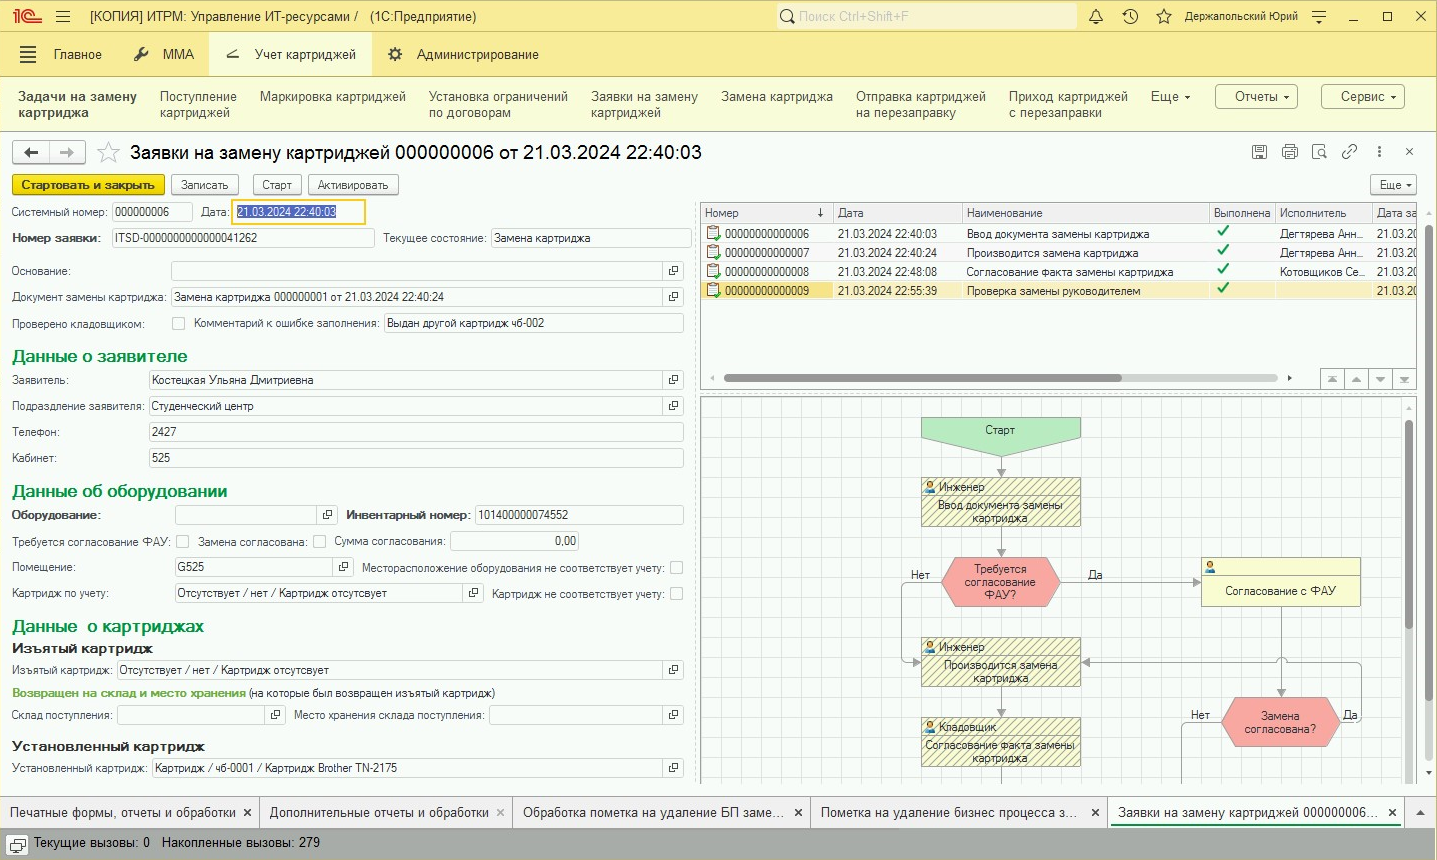
\includegraphics[width=14cm]{pictures/process.png}
% %     % \caption{}  \label{pic_label}
% % \end{figure}

